\section{Shamir Secret Sharing}
Basically it is about hiding information in a polynomial \begin{math}p\end{math}. For example, a voter chooses a random polynomial of the degree 1, which is a line. The secret is the evaluation of the polynomial in \begin{math}p(0)\end{math}. Each server receive a share, the evaluation of  \begin{math}p\end{math} in some other point. Like as server  1 receives  \begin{math}p(1)\end{math}, server 2 receives \begin{math}p(2)\end{math} and etc. To construct the line we need at most two point. One can see that if we don’t have at least 2 points then the line can be constructed in many ways, which is the same as saying we don’t know the evaluation of \begin{math}p(0)\end{math}.\\ \\
In the general case, the polynomial is chosen to be of degree \textit{t}. The scheme requires we need 
 \begin{math}t+1\end{math} points to reconstruct the secret. This means that if we have \textit{t}-servers they would not be able to obtain anything about the secret. 

\parahead{Passive corruption} is that a server (semihonest) gets access to information which the server is not entitled to, e.g. if a voter ask another voter about his information and tries to compare the information and get some more information in that way. By using secret sharing we can prevent passive corruption, because the scheme guaranties that if \textit{t}-servers are corrupted then they will not be able to gain anything.

\parahead{Active corruption} happens when the voters (malicious) try to send values that they are not supposed to send - so the voters deviate from the protocol. \\
\textcolor{red}{Ignacio: according to "Introduction to Modern Cryptography" page 503 the verifiable secret sharing scheme prevent two separate concerns on active corruption. Does this also hold for the PVSS scheme -can you please elaborate that. }

\subsection{Lagrange interpolation}
The idea is that we know some evaluations points. With Lagrange interpolation, we have a formula, with which we can reconstruct the polynomial.
The general formula, Lagrange interpolation, looks like:

\begin{defi}[Lagrange polynomial interpolation]
\begin{math}p(x)=\sum\limits_{i \in C} p(i)\lambda_i(x)\end{math}, where $\lambda_i(x)$ is defined by \begin{math} \lambda_i(x)=\prod\limits_{j\in C,j\neq i}  \frac{x-j}{i-j} \end{math}
\end{defi}

\noindent
In secret sharing scheme each server get some shares ("points") and if there are enough servers then the servers can reconstruct the secret by reconstructing the polynomial. By example we will show how the formula works.  We have a polynomial \textit{p}, where we know the evaluation of some points.

\begin{figure}[H]
    \centering
    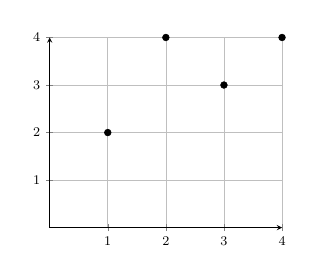
\begin{tikzpicture}[scale=0.6]
    \begin{axis}[
            grid = major,
            xmin=0, xmax=4,
            ymin=0, ymax=4,
            axis lines=center,
            axis on top=true,
            small,
            domain=0:4,
        ]
        \addplot[only marks, color = black, mark = *]
        table[meta=label] {
            x       y       label
            1       2       a
            2       4       a
            3       3       a
            4       4       a
        };
    \end{axis}
    \end{tikzpicture} 
    \caption{polynomial p}
\end{figure}

\noindent
Instead of solving the polynomial, we will start to divide the problem into smaller pieces and solve them one by one. We create a polynomial,\begin{math} \lambda_1, \lambda_2, \lambda_3\end{math} and \begin{math}\lambda_4\end{math}, one for each point from polynomial \textit{p}. These polynomial takes value 1 in one point and 0 in the other points. For example \begin{math} \lambda_1\end{math} takes 1 in 1 and 0 in 2,3 and 4.

\begin{figure}[H]
    \centering
    \captionsetup[subfigure]{labelformat=empty}
    \begin{subfigure}[b]{0.3\textwidth}
        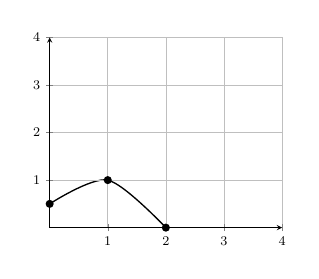
\begin{tikzpicture}[scale=0.6]
        \begin{axis}[
                grid = major,
                xmin=0, xmax=4,
                ymin=0, ymax=4,
                axis lines=center,
                axis on top=true,
                small,
            ]
            \addplot[smooth, thick, color = black, mark = *]
            table[meta=label] {
                x       y       label
                0       0.5     a
                1       1       a
                2       0       a
            };
        \end{axis}
        \end{tikzpicture} 
        \caption{approximately $\lambda_1$}
    \end{subfigure}
    \qquad % <----------------- SPACE BETWEEN PICTURES
    \qquad % <----------------- SPACE BETWEEN PICTURES
    \qquad % <----------------- SPACE BETWEEN PICTURES
    \qquad % <----------------- SPACE BETWEEN PICTURES
    \begin{subfigure}[b]{0.3\textwidth}
        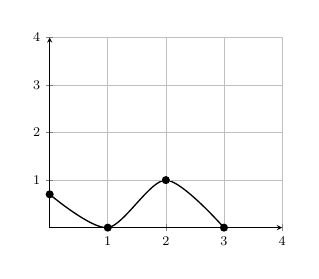
\begin{tikzpicture}[scale=0.6]
        \begin{axis}[
                grid = major,
                xmin=0, xmax=4,
                ymin=0, ymax=4,
                axis lines=center,
                axis on top=true,
                small,
            ]
            \addplot[smooth, thick, color = black, mark = *]
            table[meta=label] {
                x       y       label
                0       0.7     a
                1       0       a
                2       1       a
                3       0       a
            };
        \end{axis}
        \end{tikzpicture} 
        \caption{approximately $\lambda_2$}
    \end{subfigure}
\end{figure}

\noindent
Note that the evaluation in 0 will depend on the secret. For the sake of the drawings it is just an approximately of the point.

\begin{figure}[H]
    \centering
    \captionsetup[subfigure]{labelformat=empty}
    \begin{subfigure}[b]{0.3\textwidth}
        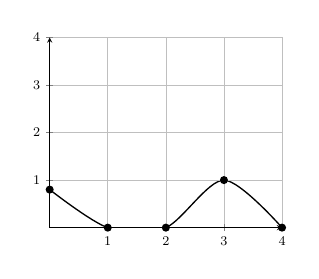
\begin{tikzpicture}[scale=0.6]
        \begin{axis}[
                grid = major,
                xmin=0, xmax=4,
                ymin=0, ymax=4,
                axis lines=center,
                axis on top=true,
                small,
            ]
            \addplot[smooth, thick, color = black, mark = *]
            table[meta=label] {
                x       y       label
                0       0.8     a
                1       0       a
                2       0       a
                3       1       a
                4       0       a
            };
        \end{axis}
        \end{tikzpicture} 
        \caption{approximately $\lambda_3$}
    \end{subfigure}
    \qquad % <----------------- SPACE BETWEEN PICTURES
    \qquad % <----------------- SPACE BETWEEN PICTURES
    \qquad % <----------------- SPACE BETWEEN PICTURES
    \qquad % <----------------- SPACE BETWEEN PICTURES
    \begin{subfigure}[b]{0.3\textwidth}
        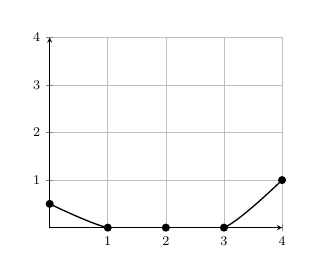
\begin{tikzpicture}[scale=0.6]
        \begin{axis}[
                grid = major,
                xmin=0, xmax=4,
                ymin=0, ymax=4,
                axis lines=center,
                axis on top=true,
                small,
            ]
            \addplot[smooth, thick, color = black, mark = *]
            table[meta=label] {
                x       y       label
                0       0.5     a
                1       0       a
                2       0       a
                3       0       a
                4       1       a
            };           
        \end{axis}
        \end{tikzpicture} 
        \caption{approximately $\lambda_4$}
    \end{subfigure}
\end{figure}

\noindent
To construct the polynomial \begin{math}p\end{math} is to take each polynomials and multiply the corresponding coefficient from \begin{math}p\end{math} and then sum the polynomials together \begin{math}2∙\lambda_1+4∙\lambda_2+3∙\lambda_3+4∙\lambda_4 \end{math}. We started with the \begin{math}\lambda\end{math} polynomial and we ended with four polynomials, which takes value 2,4,3,4 and 0 in the other points. From the sum we see that the value in the first point 2+0+0+0. It is clear this will work in the other points. 

\begin{figure}[H]
    \centering
    \captionsetup[subfigure]{labelformat=empty}
    \begin{subfigure}[b]{0.3\textwidth}
        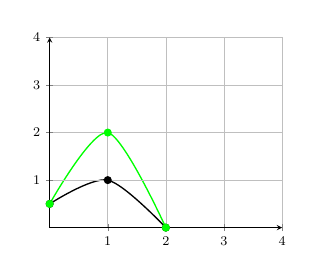
\begin{tikzpicture}[scale=0.6]
        \begin{axis}[
                grid = major,
                xmin=0, xmax=4,
                ymin=0, ymax=4,
                axis lines=center,
                axis on top=true,
                small,
            ]
            \addplot[smooth, thick, color = black, mark = *]
            table[meta=label] {
                x       y       label
                0       0.5     a
                1       1       a
                2       0       a
            };
            \addplot[smooth, thick, color = green, mark = *]
            table[meta=label] {
                x       y       label
                0       0.5     a
                1       2       a
                2       0       a
            };             
        \end{axis}
        \end{tikzpicture} 
        \caption{approximately $\lambda_1$}
    \end{subfigure}
    \qquad % <----------------- SPACE BETWEEN PICTURES
    \qquad % <----------------- SPACE BETWEEN PICTURES
    \qquad % <----------------- SPACE BETWEEN PICTURES
    \qquad % <----------------- SPACE BETWEEN PICTURES
    \begin{subfigure}[b]{0.3\textwidth}
        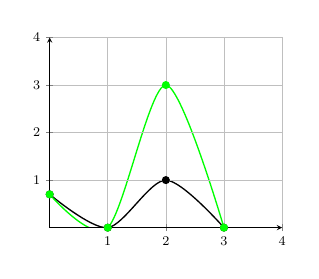
\begin{tikzpicture}[scale=0.6]
        \begin{axis}[
                grid = major,
                xmin=0, xmax=4,
                ymin=0, ymax=4,
                axis lines=center,
                axis on top=true,
                small,
            ]
            \addplot[smooth, thick, color = black, mark = *]
            table[meta=label] {
                x       y       label
                0       0.7     a
                1       0       a
                2       1       a
                3       0       a
            };
            \addplot[smooth, thick, color = green, mark = *]
            table[meta=label] {
                x       y       label
                0       0.7     a
                1       0       a
                2       3       a
                3       0       a
            };             
        \end{axis}
        \end{tikzpicture} 
        \caption{approximately $\lambda_2$}
    \end{subfigure}
\end{figure}

\begin{figure}[H]
    \centering
    \captionsetup[subfigure]{labelformat=empty}
    \begin{subfigure}[b]{0.3\textwidth}
        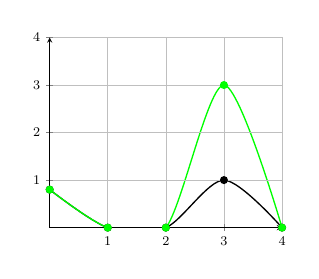
\begin{tikzpicture}[scale=0.6]
        \begin{axis}[
                grid = major,
                xmin=0, xmax=4,
                ymin=0, ymax=4,
                axis lines=center,
                axis on top=true,
                small,
            ]
            \addplot[smooth, thick, color = black, mark = *]
            table[meta=label] {
                x       y       label
                0       0.8     a
                1       0       a
                2       0       a
                3       1       a
                4       0       a
            };
            \addplot[smooth, thick, color = green, mark = *]
            table[meta=label] {
                x       y       label
                0       0.8     a
                1       0       a
                2       0       a
                3       3       a
                4       0       a
            };            
        \end{axis}
        \end{tikzpicture} 
        \caption{approximately $\lambda_3$}
    \end{subfigure}
    \qquad % <----------------- SPACE BETWEEN PICTURES
    \qquad % <----------------- SPACE BETWEEN PICTURES
    \qquad % <----------------- SPACE BETWEEN PICTURES
    \qquad % <----------------- SPACE BETWEEN PICTURES
    \begin{subfigure}[b]{0.3\textwidth}
        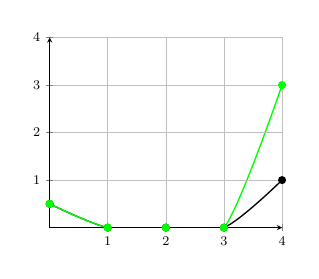
\begin{tikzpicture}[scale=0.6]
        \begin{axis}[
                grid = major,
                xmin=0, xmax=4,
                ymin=0, ymax=4,
                axis lines=center,
                axis on top=true,
                small,
            ]
            \addplot[smooth, thick, color = black, mark = *]
            table[meta=label] {
                x       y       label
                0       0.5     a
                1       0       a
                2       0       a
                3       0       a
                4       1       a
            };
            \addplot[smooth, thick, color = green, mark = *]
            table[meta=label] {
                x       y       label
                0       0.5     a
                1       0       a
                2       0       a
                3       0       a
                4       3       a
            };               
        \end{axis}
        \end{tikzpicture} 
        \caption{approximately $\lambda_4$}
    \end{subfigure}
\end{figure}


\noindent
We will now construct one of the \begin{math}\lambda\end{math}-polynomials by example, by showing it from \begin{math}\lambda_1\end{math} polynomial. 
We have the following points \begin{math}\lambda_1(1)=1, \lambda_1(2)=0, \lambda_1(3)=0 \end{math} and \begin{math} \lambda_1 (4)=0\end{math}. We take the polynomial \begin{math} (x-2)(x-3)(x-4)\end{math}, and we see that if we get correct evaluation in \begin{math}\lambda_1 (2)=0, \lambda_1 (3)=0\end{math} or \begin{math} \lambda_1 (4)=0\end{math}. To get correct evaluation in  \begin{math} \lambda_1 (1)=1\end{math} we divide by \begin{math}-6\end{math} because we see that \begin{math}(1-2)(1-3)(1-4)=-6\end{math} and then we end up with a polynomial \begin{math}\frac{(x-2)(x-3)(x-4)}{(-6)}\end{math} .  The polynomial still satisfies the conditions because when we divide zero with "something" we get zero.  The formula for constructing \begin{math}\lambda_1\end{math} 

\begin{center}
\begin{math} \lambda_1(x)=\prod\limits_{j\in C,j\neq1} \frac{x-j}{1-j} = \frac{x-2}{1-2}*\frac{x-3}{1-3}*\frac{x-4}{1-4}=\frac{(x-2)(x-3)(x-4)}{-6} \end{math}\\
\end{center}

\noindent
\begin{math} \lambda_1\end{math} gives 1 in point 1 and 0 in the other points. What this mean is that in \begin{math} \lambda_1(1)=1\end{math} and all other points  \begin{math}j (2,3,4)\end{math} we have \begin{math} \lambda_1 (j)=0\end{math}. We can construct \begin{math}\lambda_1, \lambda_2, \lambda_3\end{math} and  \begin{math}\lambda_4\end{math} in the same way.

\begin{center}
\begin{math} \lambda_2(x)=\prod\limits_{j\in C,j\neq2} \frac{x-j}{2-j} = \frac{x-1}{2-1}*\frac{x-3}{2-3}*\frac{x-4}{2-4}=\frac{(x-1)(x-3)(x-4)}{-2} \end{math}\\ \begin{math} \lambda_3(x)=\prod\limits_{j\in C,j\neq3} \frac{x-j}{3-j} = \frac{x-1}{3-1}*\frac{x-3}{3-2}*\frac{x-4}{3-4}=\frac{(x-1)(x-2)(x-4)}{-2} \end{math}\\ \begin{math} \lambda_4(x)=\prod\limits_{j\in C,j\neq4} \frac{x-j}{4-j} = \frac{x-1}{4-1}*\frac{x-3}{4-2}*\frac{x-3}{4-3}=\frac{(x-1)(x-2)(x-3)}{-6} \end{math}\\ \end{center}

\noindent
With the knowledge of the evaluation of \begin{math}p(1), p(2), p(3)\end{math} and  \begin{math}p(4)\end{math} we construct the formula for polynomial evaluation in \begin{math}p(0)\end{math}:


\noindent
\begin{infobox}[Applying Lagrange polynomial interpolation for polynomial evaluation in $0$]
We use the formula \begin{math}p(x)=\sum\limits_{i \in C} p(i)\lambda_i(x)\end{math} and we get the evaluation on some polynomial in $0$
\begin{center}
\begin{math}p(0)=p(1)∙\lambda_1+p(2)∙\lambda_2+p(3)∙\lambda_3+p(4)∙\lambda_4=2∙\lambda_1+4∙\lambda_2+3∙\lambda_3+4∙\lambda_4 \end{math}
\end{center}
\label{info:Applying_Lagrange_polynomial_interpolation}
\end{infobox}



\noindent
The idea of constructing the smaller polynomials is that we can reuse them for constructing other polynomials. From the smaller pieces and the evaluation points we can construct the polynomial from Lagrange interpolation. From the secret sharing scheme we know the degree of the polynomial is bounded. Because the voter will share its secret by choosing a random polynomial of the degree at most \textit{t}. That’s a guaranty we have from the scheme. If the degree of $p(x)$ is at most \textit{t} meaning $p(x)\leq t$. Then we need $t+1$ point to reconstruct the $p(x)$. If the degree 1 (line) then we need two points. The parable is where the degree is 2, here we need 3 points to construct
the polynomial.

\begin{figure}[H]
    \centering
    \captionsetup[subfigure]{labelformat=empty}
    \begin{subfigure}[b]{0.3\textwidth}
        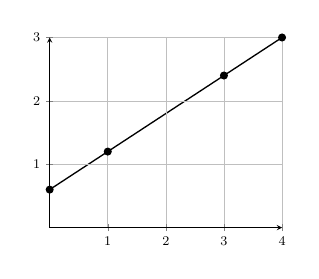
\begin{tikzpicture}[scale=0.6]
        \begin{axis}[
                grid = major,
                xmin=0, xmax=4,
                ymin=0, ymax=3,
                axis lines=center,
                axis on top=true,
                small,
            ]
            \addplot[smooth, thick, color = black, mark = *]
            table[meta=label] {
                x       y       label
                0       0.6     a
                1       1.2     a
                3       2.4     a
                4       3       a
            };
        \end{axis}
        \end{tikzpicture} 
        \caption{polynomial of degree 1}
    \end{subfigure}
    \qquad % <----------------- SPACE BETWEEN PICTURES
    \qquad % <----------------- SPACE BETWEEN PICTURES
    \qquad % <----------------- SPACE BETWEEN PICTURES
    \qquad % <----------------- SPACE BETWEEN PICTURES
    \begin{subfigure}[b]{0.3\textwidth}
        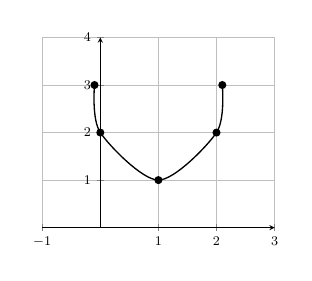
\begin{tikzpicture}[scale=0.6]
        \begin{axis}[
                grid = major,
                xmin=-1, xmax=3,
                ymin=0, ymax=4,
                axis lines=center,
                axis on top=true,
                small,
            ]
            \addplot[smooth, thick, color = black, mark = *]
            table[meta=label] {
                x       y       label
                -0.1    3       a
                0       2       a
                1       1       a
                2       2       a
                2.1     3

            };           
        \end{axis}
        \end{tikzpicture} 
        \caption{polynomial of degree 2}
    \end{subfigure}
\end{figure}


\parahead{In the PVSS protocol} we will use a simplified version of Lagrange interpolation formula. So instead of recovering the polynomium we just recover the evaluation in zero. The following will happen if take the formula \begin{math} \lambda_i(x)=\prod\limits_{j\in C,j\neq i}  \frac{x-j}{i-j} \end{math} and evaluate in zero \begin{math} \lambda_i(0)=\prod\limits_{j\in C,j\neq i}  \frac{0-j}{i-j} = \frac{j}{j-i} \end{math}. We reduce the formula by evaluating in $0$ and then one can multiply the numerator and denominator by $-1$ and then we get a the above formula.


\noindent
\begin{infobox}[Computing the coefficients for 3 tallier]
\begin{math}\lambda_1(0)=\prod\limits_{j\in C,j\neq 1} \frac{2}{2-1}  \cdot  \frac{3}{3-1} =\frac{3}{1} = 3 \end{math}\\
\begin{math}\lambda_2(0)=\prod\limits_{j\in C,j\neq 2} \frac{1}{1-2}  \cdot  \frac{3}{3-2} =\frac{1}{-1} \cdot  \frac{3}{1} =-1 \cdot  3=-3 \end{math}\\
\begin{math}\lambda_3(0)=\prod\limits_{j\in C,j\neq 3} \frac{1}{1-3}  \cdot  \frac{2}{2-3} =\frac{1}{-2} \cdot  \frac{2}{-1} =1 \end{math}\\
\textcolor{red}{Question to Ignacio: In our simpel example we have hardcoded and used these values but, if we want to compute the protocol with large values, can we still use these values or do we have to take other things into account?}
\label{info:Computing_the_coefficients}
\end{infobox}


%------------------------------------------------------------------------------------
\subsection{Homomorphic Secret Sharing}
%------------------------------------------------------------------------------------
A homomorphism is a transformation from one algebraic structure into another of the same type so that the structure is preserved. Importantly, this means that for every kind of manipulation of the original data, there is a corresponding manipulation of the transformed data.\\

\noindent 
A homomorphic encryption scheme is a crypto system that allows computations to be performed on data without decrypting it. It is an encrypting scheme which allows computations to be carried out on ciphertext, thus generating an encrypted result which, when decrypted, matches the result of operations performed on the plaintext.\\

\parahead{Homomorphic Secret Sharing} is a type of secret sharing algorithm in which the secret is encrypted via homomorphic encryption. In the PVSS scheme we use this property that one can sum the shares which are equal to the sum of the secrets.

\begin{defi}[Homomorphic Secret Sharing]
\begin{math}s\rightarrow (s_i,...,s_n)\end{math}\\
\begin{math}u\rightarrow (u_i,...,u_n) \end{math}\\
\begin{math}s+u\rightarrow (s_i+u_i,...,s_n+u_n) \end{math}\\
\textcolor{red}{Ignacio: We need a formal definition. In "Introduction to Modern Cryptography" there are explanation on Homomorphic encryption page.499. It is correct understood that we use the property of Homomorphic Secret Sharing in section 12.3 }
\end{defi}

